\documentclass{article}
\usepackage{fullpage}
\usepackage{amsmath,amssymb,amsfonts}
\usepackage{graphicx}
\usepackage{natbib}
\usepackage[colorinlistoftodos]{todonotes}
\usepackage{hyperref}
\usepackage{amsthm}
\usepackage{cleveref}

\usepackage[noend]{algpseudocode}
\usepackage{algorithm}
\usepackage{algorithmicx}

\def\R{{\mathbb{R}}}
\def\pr{{\rm Pr}}
\def\E{{\mathbb E}}
\def\X{{\mathcal X}}
\def\Y{{\mathcal Y}}
\def\H{{\mathcal H}}
\def\G{{\mathcal G}}
\def\B{{\mathcal B}}
\def\bias{{\rm bias}}
\def\supp{{\rm supp}}

\newcommand{\cB}{\mathcal{B}}
\newcommand{\I}{\mathcal{I}}
\newcommand{\samp}{S}
\newcommand{\Ex}{\mathbb{E}} % expected value operator
\newcommand{\eps}{\epsilon}
\newcommand{\sign}{\mbox{sign}}
\newcommand{\algname}{\textsc{AKNN}}

\newtheorem{theorem}{Theorem}
\newtheorem{lemma}[theorem]{Lemma}
\newtheorem{cor}[theorem]{Corollary}
\newtheorem{claim}[theorem]{Claim}
\newtheorem{defn}[theorem]{Definition}
\newtheorem{assump}{Assumption}
\newtheorem{open}{Open problem}
%\newenvironment{proof}{\noindent {\sc Proof:}}{$\Box$ \medskip}

\DeclareMathOperator*{\argmax}{arg\,max}

\newcommand{\new}[1]{{\color{red} #1}}
\newcommand{\shay}[1]{{\color{purple} {\bf Shay:} #1}}
\newcommand{\akshay}[1]{{\color{blue} {\bf Akshay:} #1}}
\newcommand{\yoav}[1]{{\color{green} {\bf Yoav:} #1}}
\title{An adaptive nearest neighbor rule for classification}

\begin{document}

\maketitle

\section{Introduction}

We introduce an adaptive nearest neighbor classification rule. Given a training set with labels $\{-1,1\}$ and a query point $x$, it makes a prediction based on the training points closest to $x$, rather like the $k$-nearest neighbor rule. However, the value of $k$ that it uses can vary from query to query. Specifically, if there are $n$ training points, then for any query $x$, the smallest $k$ is sought for which the $k$ points closest to $x$ have labels whose average is either greater than $+\Delta(n,k)$, in which case the prediction is $1$, or less than $- \Delta(n,k)$, in which case the prediction is $-1$; and if no such $k$ exists, then the label "?" us output, which corresponds to "label unknown". 
Here $\Delta(n,k) \sim \sqrt{(\log n)/k}$ corresponds to a confidence interval for the average label in the region around the query.

We study this rule in the standard framework in which all data are i.i.d.\ draws from some unknown underlying distribution $P$ on $\X \times \Y$, where $\X$ is the data space and $\Y$ is the label space. We take $\X$ to be a separable metric space, with distance function $d: \X \times \X \rightarrow \R$, and we take $\Y = \{-1,+1\}$. 
\yoav{We have two variants. The one described here, which only assumes a metric space, and the one in which we assume a euclidean space. The first is more general, the second is needed for active learning. I suggest we write the paper for case 1, and add a section at the end regarding case 2.}
\shay{Note that in the second one, where we assume a low VC dimension of the entire family of balls also allow for a faster rate (I believe that the assumptions we pick will yield a logarithmic rate in $1/\delta$). Therefore, if we also wish to discuss rates of convergence in this paper then we should consider including it.}
We can decompose $P$ into the marginal distribution $\mu$ on $\X$ and the conditional expectation of the label at each point $x$: if $(X,Y)$ represents a random draw from $P$, define $\eta(x) = \E(Y| X = x)$. In this terminology, the Bayes-optimal classifier is the rule $g^*: \X \rightarrow \{-1,+1\}$ given by
$$ g^*(x) = \sign(\eta(x)) $$
and its error rate is $R^* = \frac{1}{2}\E_{X \sim \mu} \left[1-|\mu(X)| \right]$. A variety of nonparametric classification schemes are known to have error rates that converge asymptotically to $R^*$. These include $k$-nearest neighbor (henceforth, $k$-NN) rules in which $k$ grows with the number of training points $n$ according to a suitable schedule $(k_n)$, under certain technical conditions on the metric measure space $(\X, d, \mu)$.

In this paper, we are interested in consistency as well as rates of convergence. In particular, we find that the adaptive nearest neighbor rule is also asymptotically consistent (under the same technical conditions) while converging at a rate that is at least as good as, and in some cases better than, that of $k$-NN under any schedule $(k_n)$.

Intuitively, one of the advantages of $k$-NN over nonparametric classifiers that use a fixed bandwidth or radius, such as Parzen window or kernel density estimators, is that $k$-NN automatically adapts to variation in the marginal distribution $\mu$: in regions with large $\mu$, the $k$ nearest neighbors lie close to the query point, while in regions with small $\mu$, the $k$ nearest neighbors can be further afield. The adaptive NN rule that we propose goes further: it also adapts to variation in $\eta$. In certain regions of the input space, where $\eta$ is close to $1/2$, an accurate prediction would need large $k$. In other regions, where $\eta$ is near 0 or 1, a small $k$ would suffice, and in fact, a larger $k$ might be detrimental because neighboring regions might be labeled differently. See Figure~\ref{fig:rationale} for one such example. A $k$-NN classifier is forced to pick a single value of $k$ that trades off between these two contingencies. Our adaptive NN rule, however, can pick the right $k$ in each neighborhood separately.

\begin{figure}
\begin{center}
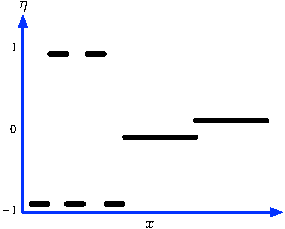
\includegraphics[width=3in]{adaptive-rationale.pdf}
\end{center}
\caption{For values of $x$ on the left half of the shown interval, the conditional probability function $\eta(x)$ is close to 0 or 1, and thus a small value of $k$ will yield an accurate prediction. Larger $k$ will not do as well, because they may run into neighboring regions with different labels. For values of $x$ on the right half of the interval, $\eta(x)$ is close to $1/2$, and thus large $k$ is essential for accurate prediction.}
\label{fig:rationale}
\end{figure}


\section{An adaptive nearest neighbor rule}

Let $(\X,d)$ be a separable metric space and let $\Y = \{-1,1\}$. Suppose we are given a labeled data set $(x^{(1)}, y^{(1)}), \ldots, (x^{(n)}, y^{(n)}) \in \X \times \Y$.

For any set $S \subset \X$, define the empirical mass of $S$ to be
\begin{equation}
\mu_n(S) = \frac{\lvert \{x^{(i)} \in S\}\rvert}{n} ,
\label{eq:empirical-mass}
\end{equation}
and define the empirical label bias of $S$ as
\begin{equation}
\bias_n(S) = \frac{\lvert\{x^{(i)} \in S: y^{(i)} = 1\}\rvert}{\lvert \{x^{(i)} \in S\}\rvert} - \frac{1}{2} = \frac{\lvert\{x^{(i)} \in S: y^{(i)} = 1\}\rvert}{n\mu_n(S)} - \frac{1}{2}.
\label{eq:empirical-bias}
\end{equation}

Let $0 < \delta < 1$ be any pre-specified confidence parameter. Given a query point $x$, we make a prediction $\{0,1,?\}$, where $?$ denotes ``don't know'', according to the following rule:
\begin{itemize}
\item Find the smallest ball $B$ centered at $x$ whose empirical bias has absolute value at least
$$ \Delta(n,k,\delta) = c_1 \sqrt{\frac{\log n + \log (1/\delta)}{k}}, $$
where $k$ is the number of points $x^{(i)}$ in $B$. The constant $c_1$ is from Lemma~\ref{lemma:bias} below.
\shay{I presume $d_0$ denotes the VC dimension of the family of all balls? 
$d_0$ should be set to $1$ in the case of the ``expected-case'' analysis}
\yoav{I suggest we push $d_0$ to the end of the paper}
\item If no such ball exists: predict ?. Otherwise, predict the majority label in $B$.
\end{itemize}
Let $g_n: \X \rightarrow \{0,1,?\}$ denote this classifier.

\section{Large deviation bounds}

Suppose that all data $(x,y)$ is obtained by independent draws from an underlying distribution $P$ on $\X \times \Y$. For $(X,Y) \sim P$, define $\mu$ to be the marginal distribution of $X$, that is,
$$ \mu(S) = \pr(X \in S) $$
for measurable sets $S$. Let $\eta$ be the conditional probability distribution of $Y$ given $x$,
$$ \eta(x) = \pr(Y = 1| X = x) .$$
For measurable $S$, let $\eta(S)$ denote the average $\eta$-value, that is,
$$ \eta(S) = \pr(Y = 1| X \in S) = \frac{1}{\mu(S)} \int_S \eta \ d \mu .$$

Suppose we draw $n$ points $(x^{(1)}, y^{(1)}), \ldots, (x^{(n)}, y^{(n)})$ from $P$. If $n$ is reasonably large, we would expect the empirical mass $\mu_n(S)$ of any set $S \subset \X$, as defined in (\ref{eq:empirical-mass}), to be close to its probability mass under $\mu$. The following lemma, from \cite{ChaudhuriDasgupta2010}, quantifies one particular aspect of this.
\begin{lemma}[\cite{ChaudhuriDasgupta2010}, Lemma 7]
There is a universal constant $c_0$ such that the following holds. Let $\B$ be any class of measurable subsets of $\X$ of VC dimension $d_0$. Pick any $0 < \delta < 1$. Then with probability at least $1-\delta^2/2$ over the choice of $(x^{(1)}, y^{(1)}), \ldots, (x^{(n)}, y^{(n)})$, for all $B \in \B$ and for any integer $k$, we have
$$ \mu(B) \geq \frac{k}{n} + \frac{c_0}{n} \max \left( k, d_0 \log \frac{n}{\delta} \right)
\ \ \implies \ \ 
\mu_n(B) \geq \frac{k}{n} .$$
\label{lemma:points-in-balls}
\end{lemma}

Likewise, we would expect the empirical bias of a set $S \subset \X$, as defined in (\ref{eq:empirical-bias}), to be close to its true bias,
$$ \bias(S) = \frac{\pr(Y = 1, X \in S)}{\pr(X \in S)} - \frac{1}{2} .$$
This is defined when $\mu(S) > 0$ and lies in the range $[-1/2,1/2]$.

\begin{lemma}
There is a universal constant $c_1$ for which the following holds. Let $\B$ be a class of subsets of $\X$ with VC dimension $d_0$. Pick any $0 < \delta < 1$. Then with probability at least $1-\delta^2/2$ over the choice of $(x^{(1)}, y^{(1)}), \ldots, (x^{(n)}, y^{(n)})$, for all $B \in \B$,
  $$ \left| \bias_n(B) - \bias(B) \right| \ \leq \ \Delta(n, k(B)) $$
where $k(B) = |\{i: x^{(i)} \in B\}|$ is the number of points inside $B$ and 
\begin{equation}
\Delta(n,k) = c_1 \sqrt{\frac{d_0 \log n + \log (1/\delta)}{k}} .
\label{eq:delta-defn}
\end{equation}
\label{lemma:bias}
\end{lemma}

\Cref{lemma:bias} is a special case of a uniform convergence bound for conditional probabilities (\Cref{thm:UCECM}) 
that we present and prove in \Cref{sec:ucecm}.




\section{Fine-grained analysis and universal consistency}
\label{sec:universal-consistency}

Define the support of the marginal distribution $\mu$ to be
$$ \supp(\mu) = \{x \in \X: \mbox{$\mu(B(x,r)) > 0$ for all $r > 0$}\} .$$

For any $x \in \supp(\mu)$ and $p > 0$, let $r_p(x)$ denote the smallest radius such that the probability mass of $B(x, r_p(x))$ is at least $p$:
$$ r_p(x) = \inf \{r > 0: \mu(B(x,r)) \geq p \} .$$
Then $\mu(B(x,r_p(x))) \geq p$.

We now characterize the region of $\X$ that $\algname$ is likely to correctly classify as having label $1$, given $n$ training points. It is the set $\X^+_n$ of points $x \in \supp(\mu)$, with $\eta(x) > 1/2$, for which there exists $p_x > 0$ such that:
\begin{itemize}
\item $\eta(B(x,r_{p_x}(x))) \geq \frac{1}{2} + c_2 \sqrt{\frac{\log (n/\delta)}{np_x}}$, where $c_2 = \max(2c_1, 1/2) \sqrt{1+c_0}$. 
\item $\eta(B(x,r)) \geq 1/2$ for all $0 < r \leq r_{p_x}(x)$. 
\end{itemize}
The set $\X^-_n$ can be defined symmetrically, as consisting of $x \in \supp(\mu)$ with $\eta(x) < 1/2$, and for which there exists $p_x > 0$ such that:
\begin{itemize}
\item $\eta(B(x,r_{p_x}(x))) \leq \frac{1}{2} - c_2 \sqrt{\frac{\log (n/\delta)}{np_x}}$. 
\item $\eta(B(x,r)) \leq 1/2$ for all $0 < r \leq r_{p_x}(x)$. 
\end{itemize}

\begin{lemma}
Fix any $x \in \X^+_n \cup \X^-_n$. Pick $n$ training points at random from $P$. With probability at least $1-\delta^2$ over the choice of training data, the adaptive $k$-NN rule will predict 1 if $x \in \X^+_n$, or $0$ if $x \in \X^-_n$.
\label{lemma:good-sets}
\end{lemma}


Based on this result, it makes sense to define the {\it effective boundary} when there are $n$ data points as 
$$ \partial_n = \X \setminus (\X^+_n \cup \X^-_n) .$$
Then we have the following bound on the error rate of the adaptive nearest neighbor classifier.
\begin{theorem}
Pick any $0 < \delta < 1$. With probability at least $1-\delta$ over the choice of training points,
$$ \pr_{X}(g_n(X) \neq g^*(X)) \ \leq \ \delta + \mu(\partial_n) .$$
Here $g_n$ is the adaptive nearest neighbor classifier based on the $n$ training points and $g^*$ is the Bayes-optimal classifier. \shay{The quantification over $\delta$ confuses me; note that the adaptive nearest neighbor classifier $g_n$ gets $\delta$ as an input (because the threshold $\Delta(n,k)$ does).} 
\label{thm:general-error-bound}
\end{theorem}


It follows, using the same argument as in \cite{ChaudhuriDasgupta2014}, that the adaptive nearest neighbor rule is universally consistent as long as the metric space $(\X, d, \mu)$ satisfies Lebesgue's differentiation condition: that is, for any bounded measurable $f: \X \rightarrow \R$ and for $\mu$-almost\footnote{I.e., the set of points which does not satisfy the condition has measure $0$ under $\mu$.} every $x$,
$$ \lim_{r \downarrow 0} \frac{1}{\mu(B(x,r))} \int_{B(x,r)} f \ d\mu = f(x) .$$
This holds in any finite-dimensional normed space, or any doubling metric space.
\shay{In order for consistency to hold, 
one should tune $\delta= \delta(n)$ such that $\delta(n)\to_{n\to\infty} 0$.
(note that $\delta$ is a parameter of our algorithm, unlike in \cite{ChaudhuriDasgupta2014}, where $\delta$
was just defined for sake of analysis). }



\section{High-probability convergence}

In this section, we make a further assumption that allows us to strengthen \Cref{thm:general-error-bound}, tightly quantifying over all query points simultaneously. 
\begin{assump}
\label{assump:VCallballs}
The family of all balls in $(\X, d)$ has VC dimension $d_0 < \infty$.
\end{assump}
This is motivated by finite-dimensional Euclidean space $\mathbb{R}^{D}$, where \Cref{assump:VCallballs} is satisfied with $d_0 = D+1$ \citep{dudley79}. Given such a $d_0$ and parameter $\delta$, define $\kappa_{n, \delta} := d_0 \log n + \log (1/\delta)$. 
For $s \in \{ -1, +1 \}$, define the following quantities that depend on the algorithm's lone confidence parameter $\delta$:
\begin{align*}
\X^{s}_n (\delta)
:= \Bigg\{
x \in \supp(\mu) : s \eta(x) > 0 , \exists p_x > 0 \text{ s.t. } 
&s \eta(B(x,r_{p_x}(x))) \geq 2 c_2 \sqrt{\frac{ \kappa_{n, \delta} }{n p_x}}
\quad\text{and}\quad \\
&s \eta(B(x,r)) \geq 0 \quad\forall r \in (0, r_{p_x}(x)]
\Bigg\}
\end{align*}
where $c_2 = \max(2c_1, \frac{\varphi}{2} ) \sqrt{1 + c_0}$ for $\varphi := \frac{1}{2} (1 + \sqrt{5})$.
Also define 
$$ \partial_n (\delta) = \X \setminus (\X^+_n (\delta) \cup \X^-_n (\delta)) $$
Then our main convergence rate result in this scenario shows that the measure of the effective boundary bounds the convergence of $\algname$.


\begin{theorem}\label{thm:fastrate2}
Let $\delta$ be the confidence parameter of the $\algname$ algorithm, and suppose \Cref{assump:VCallballs} holds with VC dimension $d_0$.
Then, with probability at least $1-\delta$ over the choice of training points,
\[ \pr_{X}(g_n(X) \neq g^*(X)) \ \leq \ \mu(\partial_n (\delta)) .\]
Here $g_n$ is the adaptive nearest neighbor classifier based on the $n$ training points and $g^*$ is the Bayes-optimal classifier. 
\end{theorem}

\akshay{Is it worth showing that \Cref{thm:fastrate2} is tight, e.g. the instance-dependent lower bounds of \cite{ChaudhuriDasgupta2014}?}



The difference with \Cref{thm:general-error-bound} is that the $\delta$ term is removed.

{\it To summarize, for convergence in expectation we bound the error by $\delta + \mu(\partial_n)$,
and for convergence with high probability we bound it by $\mu(\partial_n)$.}
So, in order to get explicit bounds in both settings, we need to figure out how $\mu(\partial_n)$ decays under natural assumptions. It would be nice if we could get something like 
\[\mu(\partial_n (\delta)) \leq \mathrm{poly}\left(\log(1/\delta), n\right),
\]
with hidden constant depending on the assumptions we make.
\akshay{Here I think the smoothness condition introduced in \cite{ChaudhuriDasgupta2014} is relevant.}


\section{Rates of convergence}


\subsubsection{Shay's comments}

There are two natural settings we could consider: (i) convergence in expectation, and (ii) convergence with high probability.
Convergence in expectation boils down to \Cref{thm:general-error-bound} in the previous section.
For convergence with high probability we further assume that the VC dimension of the family of all balls is bounded. 
Note that in this case we should also change the definition of $\Delta(n,k)$  in the algorithm so that it has the right dependence on the VC dimension. \akshay{It's already correct in the initial definition of the algorithm, but not consistent in the definitions of $\X^{\pm}_n$.} What we can prove in this case is \Cref{thm:fastrate} (stated in a subsection below), 
which can also be phrased more similarly to \Cref{thm:general-error-bound}) as in \Cref{thm:fastrate2}.



\subsubsection{Akshay's notes}


\subsubsection{Sanjoy's notes}
We now provide finite-sample rates of convergence of the adaptive nearest neighbor rule. For simplicity, we give convergence rates that are specific to any query point $x$ and that depend on a suitable notion of the ``margin'' of distribution $P$ around $x$.

Pick any $p, \gamma > 0$. We define a point $x \in \X$ as $(p, \gamma)$-salient if 
\begin{itemize}
\item either $\eta(x') \geq 1/2 + \gamma$ for all $x' \in B(x, r_p(x))$
\item or $\eta(x') \leq 1/2 - \gamma$ for all $x' \in B(x, r_p(x))$.
\end{itemize}
If $\eta$ and $\mu$ are continuous then for any $x \in \X$ with $\eta(x) \neq 1/2$, there must be some sufficiently small $p, \gamma > 0$ for which this is true.

Let $S_{p, \gamma}$ be the set of all $(p, \gamma)$-salient points. We then define the {\it margin} of any $x \in \X$ as
$$ m(x) = \max_{S_{p, \gamma} \ni x} p \gamma^2 .$$
Notice that if 
$$ n \geq \frac{1}{m(x)} \log \frac{1}{m(x)} ,$$
then $x \in \X_n^+ \cup \X_n^-$, as defined in Section~\ref{sec:universal-consistency}, and thus $x$ is very likely to be correctly classified by the adaptive nearest neighbor rule, given a training set of $n$ points.
\shay{Should $\gamma,p$ depend on $\delta$ for this containment to hold? Note that the definitions of $\X_n^+,\X_n^-$ do depend on $\delta$.}
\akshay{Agreed, as in \Cref{thm:fastrate2}.}

\subsubsection{Earlier notes}

In order that a point $x$ be classified correctly for a small value of $n$ it suffices that there is a ball $B$ centered at $x$ with significant bias and significant probability. More precisely, if there is a ball of probability $p$ around $x$ for which there is a uniform bias of $\gamma$ then probability that the adaptive NN rule is incorrect 
on $x$ is $\exp(-c k \gamma^2) \approx \exp(-c p n \gamma^2)$

We formalize this as follows.

Let $\X_{\alpha}^+$ be the set of points $x \in \X$ such that there exist $p,\gamma>0$ such that $p \gamma^2 \geq \alpha$ and  $\forall x' \in B(x,p)$ $\eta(x')\geq \gamma$. $\X_{\alpha}^-$ is defined similarly.

Then we have the following theorem:
\begin{theorem}\label{thm:fastrate}
For all $\alpha>0$ and all $x \in \X_{\alpha}^+ \cup \X_{\alpha}^-$ the probability that $\algname$ predicts incorrectly on $x$ is upper bounded by $\exp(-c n \alpha)$.
\end{theorem}


\section{Related Work}




\section{Uniform Convergence of Empirical Conditional Measures}
\label{sec:ucecm}


\subsection{Formal Statement}

Let $p$ be a distribution over $X$, let $\cB$ be a collection of events, and let $A$ be an event.
Assume that $\cB$ has a finite VC dimension $d_0$.
Consider $n$ independent samples from~$p$, denoted by $x_1,\ldots,x_n$.
We would like to estimate $p(A \vert B)$ simultaneously for all $B\in \B$.
It is natural to consider the empirical estimates:
\[p_n(A\vert B)=\frac{\sum_i 1_{[x_i\in A \cap B]}}{\sum_i 1_{[x_i\in B]}}.\]
We study how well these estimates provide a good approximation to $p$.

To demonstrate the kinds of statements we would like to derive,
consider the case where there is only one event $B$ in $\cB$, 
and set $k(B)=\sum_i 1_{[x_i\in B]}$.
A Chernoff bound implies that conditioned on the event $k(B)>0$, 
the following holds with probability at least $1-\delta$:
\begin{equation}\label{eq:chernoff}
\left\lvert p(A\vert B) - p_n(A \vert B) \right\rvert \leq \sqrt{\frac{2\log(1/\delta)}{k(B)}}.
\end{equation}
To derive it use that conditioned on $x_i\in B$, the event $x_i\in A$ has probability $p(A\vert B)$, 
and therefore the random variable ``$k(B)\cdot p_n(A \vert B)$'' has distribution $\mbox{Bin}(k(B), p(A\vert B))$.

Note that the bound on the probability in \Cref{eq:chernoff} depends on $k(B)$
and therefore is random.
We stress that this is the type of statement we want:
the more samples belong to $B$, the more certain we are with the empirical estimate.

We would like to prove something like this:
\begin{theorem}[A too-good-to-be-true UCECM]\label{thm:toogood}
The following event occurs with probability at least $1-\delta$:
\[\left(\forall B\in\B\right):\left\lvert p(A \vert B) - p_n(A \vert B) \right\rvert \leq O\left(\sqrt{\frac{d_0 \log(1/\delta)}{k(B)}}\right),\]
where $k(B) = \sum_{i=1}^n 1[x_i\in B]$.
\end{theorem}
\Cref{thm:toogood} is, unfortunately, false. 
As an example, consider the probability space defined by drawing uniformly $x\sim[n]$,
and then coloring $x$ by $c_x\in\{\pm 1\}$ uniformly.
For each $i$ let $B_i$ denote the event that~$i$ was drawn,
and let $A$ denote the event that the drawn color was  $+1$.
(formally, $B_i = \{i\}\times\{\pm 1\}$, and $A=[n]\times\{+1\}$).
One can verify that the VC dimension of $\B=\{B_i : i\leq n\}$ is $1$.

\Cref{thm:toogood} fails in this setting:
indeed, if we sample $n$ times from this space 
then with a constant probability there will be some  $j$
that is assigned with the same color in each sample,  say $+1$, 
and will be picked some $\Theta(\log n/\log\log n)$ times\footnote{{This follows from analyzing the maximal bin
in a uniform assignment of $\Theta(n)$ balls into $n$ bins~\cite{bins}}}.
Therefore, $p_n(A\vert B_i) = 1$, $p(A\vert B_i)=1/2$,
and $1-(1/2) \gg \sqrt{\log\log n/\log n}$.

We prove the following (slightly weaker) variant, the main result of this section:
\begin{theorem}[UCECM]\label{thm:UCECM}
The following event occurs with probability at least $1-\delta$:
\[\left(\forall B\in\B\right):\left\lvert p(A \vert B) - p_n(A \vert B) \right\rvert \leq 
\sqrt{\frac{k_0}{k(B)}},\]
where $k_0 = 200 \left(d_0 \log(3n) + \log(1/\delta)\right)$, and $k(B) = \sum_{i=1}^n 1[x_i\in B]$.
\end{theorem}

\paragraph{Discussion.}
%\shay{Analyze this comparison more clearly.
%I hope we can derive a statement like:
%our bound becomes meaningful
%for $B$ such that $p(B)\geq d\log n/n$
%but the naive bound requires $p(B)\geq \sqrt{d/n}$.}

\Cref{thm:UCECM} can be combined with the following uniform convergence 
variant to yield a bound on the minimal $n$ for which $p_n(A \vert B)$ 
is a non-trivial approximation of $p(A \vert B)$
(as explained below, this $n$ is some $\tilde O\left(1/p(B)\right)$).
\shay{Is the following lemma is essentially equivalent to \Cref{lemma:points-in-balls}?}
\begin{lemma}\label{lem:uconeside}
Set $k_0$ like in \Cref{thm:UCECM}. Then with probability at least $1-\delta$:
\[
(\forall B\in \B):~ k(B) \geq \frac{1}{4}np(B) - {k_0}.
\]
\end{lemma}
This implies that if $n$ is large enough so that $p(B)=\tilde\Omega(k/n)=\tilde\Omega\left(\frac{d_0}{n}\right)$
then the empirical estimate $p_n(A\vert B)$ provides a decent approximation.
In the context of specialists, this means that the empirical
biases provide meaningful estimates of the true biases 
for specialists whose measure is $\tilde\Omega\left(\frac{d_0}{n}\right)$.
Note the resemblance with the learning rate in realizable settings.
%
%indeed, it implies that roughly $p(B)\pm \sqrt{d/n}$ 
%empirical points from the sample are will indeed belong to $B$
%(with high probability), and so, once $n$ is sufficiently large,
%one can replace the radius of the confidence interval by 
%$\Theta\left(\sqrt{\frac{d\log n}{p(B)n - \sqrt{dn}}}\right)$, 
%which is for a large $n$ roughly $\sqrt{\frac{d\log n}{p(B)n}}$.

A relevant remark is that a weaker statement than \Cref{thm:UCECM}
can be derived as a corollary of the classical uniform convergence
result~\citep{V82}. 
Indeed, since the VC dimension of $\{B\cap A : i\in \I\}$ is at most $d_0$, it follows that 
\[p_n(A\vert B)\approx\frac{p(A\cap B) \pm \sqrt{d_0 / n}}{p(B)\pm \sqrt{d_0 / n}}.\]
However, this bound guarantees non-trivial estimates only once $p(B)$ is roughly $\sqrt{d_0  / n}$.
This is similar to the learning rate in the agnostic learning.

Another practical advantage of the uniform convergence bound in \Cref{thm:UCECM} is its dependence on $k(B)$,
which may be thought of as a ``lucky-case'' bound:
if (by ``luck'') many points from the sample belong to $B$ 
then $p_n(A\vert B)$ is a good estimate of $p(A\vert B)$.



\subsection{Proof of \Cref{thm:UCECM}}

\subsubsection{Overview}
The idea is to follow the standard argument due to~\cite{vapnik} 
which derives the standard uniform convergence result (and to modify it accordingly). 
We follow the exposition of~\cite{anthony}:
consider a double-sample of size $2n$ from~$p$, denoted by $x_1,\ldots,x_{2n}$.
Let $S_1$ denote the first half of the sample and $S_2$ the second.
Define $E_1$ to be the event whose probability we want to bound:
\[E_1 = \left\{ S_1\in X^n : (\exists B\in \B):~ 
\left\lvert p(A \vert B) - p_{n,1}(A \vert B) \right\rvert > 
\sqrt{\frac{k_0}{k_{1}(B)}} \right\},\]
where $p_{n,1}$ is the empirical measure induced by $S_1$, 
and $k_{1}(B)=\sum_{i=1}^n 1[x_i\in B]$ ($p_{n,2}, k_{2}$ are defined similarly).
Let $E_2$ denote the event
\[E_2 = 
\left\{
S_1S_2\in X^{2n} : (\exists B\in\B):~
\left\lvert p_{n,1}(A \vert B)   -  p_{n,2}(A \vert B) \right\rvert >  
{\frac{1}{2}}\sqrt{\frac{k_0}{k(B)}}
\right\},
\]
where $k(B) = k_{1}(B)+k_{2}(B)$.
The strategy is showing that $\Pr[E_1]$ is small by reducing it to showing that $\Pr[E_2]$ 
is small, and then to show that the latter is small using a standard \emph{symmetrization} argument. 
For the first part, we would like to argue like in~\cite{anthony}, that
\begin{equation}\label{eq:anthony} 
(\forall S_1\in E_1): \Pr_{S_2}[S_1S_2\in E_2]\geq \frac{1}{100}.
\end{equation}
Indeed, since $S_1,S_2$ are independent, this implies that $\Pr[E_2 \vert E_1]\geq\frac{1}{100}$ 
	and therefore that 
	\[\Pr[E_1] = \frac{\Pr[E_2\land E_1]}{\Pr[E_2 \vert E_1]}\leq 100\Pr[E_1\land E_2] \leq 100\Pr[E_2],\] 
	which yields the reduction.

However, \Cref{eq:anthony} does not necessarily hold: indeed assume that $\B=\{B\}$ contains
	a single set $B$ such that $p(B) \ll \frac{1}{n}$ is tiny and $p(A \vert B) = \frac{1}{2}$. 
	Now, let $S_1\in E_1$, thus
	\[
	\left\lvert p(A \vert B) - p_{n,1}(A \vert B) \right\rvert > 
	\sqrt{\frac{k_0}{k_{1}(B)}}.
	\]
	Now, since $p(B) \ll \frac{1}{n}$ then $B\cap S_2 = \emptyset$ with high probability.
	This means that $p_{n,2}(\cdot \vert B)$ is undefined and in particular that $S_1S_2\notin E_2$ 
	with high probability over the choice of $S_2$.

%
%However, \Cref{eq:anthony} does not necessarily hold: indeed consider
%	$S_1\in E_1$ such that there is a single $B$ for which 
%\[
%\left\lvert p(A \vert B) - p_{n,1}(A \vert B) \right\rvert > 
%\sqrt{\frac{k_0}{k_{1}(B)}}
%\]
%and further assume that 
%\begin{itemize}
%\item[(i)] $B$ has a tiny measure, say $p(B) \leq 1/n$,
%\item[(ii)] $p(A\vert B)= 1/2$, and
%\item[(iii)] $p_{n,1}(A\vert B) = 0$.
%\end{itemize}
%Therefore, $k_2(B)=1$ with a constant probability (at least $1/4$)
%and so $p_{n,2}(A \vert B)=p_{n,1}(A \vert B)$ 
%with probability at least~$\frac{1}{8}$ (which implies in particular that ).

To get around this, we introduce an auxiliary event $F$, defined by
\[F = \left\{S_1\in X^{n} : (\forall B\in\B): p_{n,1}(B) \geq \frac{k_0}{n} \implies p(B)\geq \frac{p_{n,1}(B)}{4}\right\}. \]
Note that $F$ discards the problematic example from above 
(by constraining every $B$ that witnesses $E_1$ to have a large probability). 
The following lemma, which can be seen as a converse to the \Cref{lemma:points-in-balls}, 
shows that $F$ is a typical event (i.e.\ has a large probability):
\shay{Maybe move this lemma to after \Cref{lemma:points-in-balls}}
\begin{lemma}\label{lem:Fistypical}
Let $\B$ be any class of measurable subsets of $\X$ of VC dimension $d_0$. Pick any $0 < \delta < 1$. Then with probability at least $1-\delta/2$ over the choice of $(x^{(1)}, y^{(1)}), \ldots, (x^{(n)}, y^{(n)})$, for all $B \in \B$ and for any integer $k$, we have
\[ p_n(B) \geq \frac{k_0}{n}
\ \ \implies \ \ 
p(B) \geq \frac{p_n(B)}{4},\]
where $k_0 = 200 \left(d_0 \log(3n) + \log(1/\delta)\right)$.
\end{lemma}

\Cref{lem:Fistypical} allows us to replace \Cref{eq:anthony} with the following:
\begin{lemma}\label{lem:reduction}
If $\Pr[E_1]\geq \delta$ then 
\begin{enumerate}
\item $\Pr[E_1\cap F] \geq \frac{1}{2}\Pr[E_1]$, and
\item $(\forall S_1\in E_1\cap F): \Pr_{S_2}[S_1S_2\in E_2] \geq \frac{1}{8}$. 
\end{enumerate}
\end{lemma}
We defer the proof of \Cref{lem:reduction} to a later section, 
and assume it for now towards proving \Cref{thm:UCECM}.

\Cref{lem:reduction} yields the following win-win situation:
either $\Pr[E_1] \leq \delta$ and we are done, or:
\[\frac{\Pr[E_2]}{\Pr[E_1]} \geq  \frac{\Pr[E_2]}{2\Pr[E_1\cap F]} \geq \frac{\Pr[E_2 \vert E_1\cap F]}{2} \geq \frac{1}{16}
\implies  \Pr[E_1]\leq 16\Pr[E_2],\]
where the first inequality uses the first item of \Cref{lem:reduction}, 
the second inequality follows by definition of conditional probability,
and the last inequality is implied by the the second item of \Cref{lem:reduction}.


We proceed to the standard symmetrization argument
that establishes $\Pr[E_2]\leq\delta/16$. 
Instead of sampling $S_1S_2\sim p^{2n}$,
consider the following equivalent process:
\begin{itemize}
\item[(i)] Sample $S\sim p^{2n}$.
\item[(ii)] Partition $S$ uniformly into two subsamples $S_1,S_2$, each of size $n$.
\end{itemize}
The following lemma implies that $\Pr[E_2]\leq \delta/16$, and finishes the proof.
\begin{lemma}\label{lem:e2}
For every $S\in X^{2n}$
\[\Pr_{S\to S_1S_2}\left[S_1S_2\in E_2\right]\leq \frac{\delta}{16},\]
where the randomness is over the uniform partitioning
of $S$ into $S_1,S_2$.
\end{lemma}
\qed

\subsubsection{Proof of \Cref{lem:Fistypical}}
\Cref{lem:Fistypical} follows from the standard uniform convergence bound with
the difference of using the multiplicative Chernoff bound instead
of the additive bound:
consider a double sample $S=(\samp_1,\samp_2)\sim p^{2n}$.
Let~$F_1 = \bar F$ denote the event whose probability we want to bound:
\[
F_1 =\left\{ S_1\in X^n : (\exists {B\in\B}):
  p_{n,1}(B) \geq \frac{k_0}{n} \mbox{ and } p(B) < \frac{p_{n,1}(B)}{4}\right\}, 
\]
and let $F_2$ denote the event:
\[
F_2 = 
\left\{ S_1S_2\in X^{2n} : (\exists {B\in\B}):
  p_{n,1}(B) \geq \frac{k_0}{n} \mbox{ and } p_{n,2}(B) < \frac{p_{n,1}(B)}{2}\right\}.
\]
The proof is an immediate consequence of the next two lemmas:
\begin{lemma}\label{lem:aux11}
$\Pr[F_1]\leq 10\Pr[F_2].$
\end{lemma}
\begin{lemma}\label{lem:aux12}
$\Pr[F_2]\leq \delta/20.$
\end{lemma}
\begin{proof}[Proof of Lemma~\ref{lem:aux11}]
It suffices to show that $\Pr[F_2 \vert F_1]\geq 1/10$.
	Indeed, this would imply that $\Pr[F_1] \leq 10\Pr[F_1 \cap F_2]\leq 10\Pr[F_2]$.
	Since $S_2$ and $S_1$ are independent it suffices to show that for all $S_1\in F_1$:
	\[\Pr_{S_2\sim p^n}\left[(S_1,S_2)\in F_2\right] \geq 1/10.\]
	Let $S_1\in F_1$, and let $B\in\B$ such that $p_{n,1}(B)\geq\frac{k_0}{n}$ and $p(B)\leq \frac{p_{n,1}(B)}{4}$.
	We show that $p_{n,2}(B)\leq \frac{p_{n,1}(B)}{2}$ with probability at least~$\frac{1}{10}$.
	Case (i): if $p(B) < 1/2n$ then 
\[
\Pr\left[ p_{n,2}(B) > \frac{p_{n,1}(B)}{2}\right]=\Pr\left[ k_{2}(B) > \frac{k_{1}(B)}{2}\right]
\leq
\Pr\left[ k_{2}(B) > 0 \right]
\leq np(B) < 1/2 < 9/10.
\]
Case (ii): else, if $p(B) \geq 1/2n$, 
	then by the multiplicative\footnote{We use here the following version: if $X=\sum_i X_i$, where the $X_i$'s are independent 0/1 random variables and $\beta\geq 1$ then $\Pr[X\geq (1+\beta)\mu] \leq \exp(\frac{-\beta^2}{2+\beta}\mu)$, where $\mu=\Ex[X]$ (see for example \cite{}).}:
\[
\Pr\left[ k_{2}(B) > \frac{k_{1}(B)}{2}\right]
\leq
\Pr\left[ k_{2}(B) > 2p(B)\cdot n\right]
\leq
\exp\left( \frac{-p(B)\cdot n}{3}\right)\leq \exp(-1/6)\leq 9/10.
\]

So, conditioned on $F_1$, 
the event $F_2$ occurs with probability at least $1/10$.
\end{proof}

\begin{proof}[Proof of Lemma~\ref{lem:aux12}]
We use a symmetrization argument: instead of sampling $\samp_1$ and then $\samp_2$,
	first sample $\samp=\samp_1\cup \samp_2$ and then partition it into two equal parts 
	$\samp_1$ and $\samp_2$ uniformly at random.
	Now, for a fixed $\samp$ what is the probability (over the random partition) that $F_2$ occurs?
	Let $\B|_{\samp} = \{B|_{\samp} : B\in\B\}$.
	It suffices to show that the event
\[F_2|_{\samp} = 
\left\{ \{S_1,S_2\}:
\exists {B\in\B|_{\samp}}:
  p_{1}(B)\geq \frac{k_0}{n} \mbox{ and } p_{2}(B) < \frac{p_{1}(B)}{2}
  \right\}
\]
has probability at most $\delta/10$ over the partition of $\samp$ into $\samp_1,\samp_2$.
To this end we use a union bound. 
	We only need to consider $B$'s in $\B|_{\samp}$ such that $k(B) > k_0$, where $k(B) = k_{1}(B)+ k_{2}(B)$. 
	Fix such a $B$; without loss of generality assume that the first $k(B)$ points 
	out of the~$2n$ points in $S$ are in $B$. 	For every $i\leq k(B)$, let $X_i$ denote 
	the indicator of the event that the $i$'th point in $S$ was drawn into $S_2$.
	Set~$X=\sum_{i=1}^{k(B)}X_i$.
	Note that $B$ causes $F_2|_{\samp}$ to occur if and only if $X\leq \frac{k(B)}{3}$.
	We would like to use a Chernoff bound to bound the probability of this event; 
	however this bound does not directly apply here as the $X_i$'s are not independent:
	indeed $S_2$ is generated via a sampling of $n$ points {\it without replacements} from $S$.
	Nevertheless, Hoeffding (\cite{H63}, Section 6) established\footnote{Theorem 4 in \cite{H63} shows 
	that any tail bound which is based on the moment-generating function (such as Chernoff bounds) applies to sampling-without-		replacement. \shay{Perhaps move this discussion to a section dedicated to tehcnical background.}} that Chernoff bounds apply also in this setting. Therefore:
%	and therefore
%	To analyze this event define a random variable $Y=\sum_{i=1}^{k(B)}Y_i$,
%	where the $Y_i$'s are independent Bernoulli random variables with probability $1/2$. 
%	Its moment-generating function upper-bounds that of $X$, i.e. $\evp{\exp(tX)}{} \leq \evp{\exp(tY)}{}$ 
%	(\cite{H63}, Thm. 4), 
%	so we can bound the tail probability $\Pr\left[X\leq k(B)/3\right]$ using a Chernoff bound on $Y$:
%\footnote{We repeatedly use this standard trick of relaxing sampling-without-replacement tail bounds based on moment-generating functions to their with-replacement counterparts in what follows.} 
%\yoav{Akshay, I can see how this argument works for a single ball $B$,
%  but not how it would work for a uniform bound over a set of balls.}
%\akshay{Yoav, where is the issue? I believe the proof from the line ``Fix such a $B$" (before this comment inline) to ``By Sauer's Lemma" is for a fixed $B$, then the standard uniform bound applies over the Sauer class $B\mid_S$. And similarly for the other applications of Chernoff to without-replacement in this writeup.}
%\shay{Here we should refer to the statement that sampling without repetitions is more concentrated.}
%\yoav{This comment by shay appears verbatim in three different
%  places. Should all of them be there? (instead of uncommenting
%  comments, change the newcommands that create them).}
\[
\Pr\left[X\leq \frac{k(B)}{3}\right] =\Pr\left[Y- \frac{k(B)}{2} < -\frac{k(B)}{6}\right]
						\leq \exp\left(-2\left(\frac{1}{6}\right)^2k(B)\right) 
						< \exp\left(-\frac{k_0}{100}\right)
\]
(where the last inequality is because $k(B) > k_0$).
By the Sauer-Shelah-Perles Lemma,
the number of distinct restrictions in $B|_S$ is at most $\left(\frac{2en}{d}\right)^d$, and therefore 
\[\Pr[F_2]\leq \left(\frac{2en}{d}\right)^d\exp\left(-\frac{k_0}{100}\right).\]
Since $k_0\geq 200\left(d\log(3n) + \log(1/\delta) \right)$, it follows
that this probability is at most $\delta/20$.
\end{proof}


\subsubsection{Proof of \Cref{lem:reduction}}

\paragraph{Item 1.}
Assume that $\Pr[E_1]\geq \delta$.
We begin with the first item:
By \Cref{lem:Fistypical} we have that $\Pr[F]\geq 1-\frac{\delta}{2}$.
Therefore,
\[\Pr[E_1\cap F] \geq \Pr[F] - (\Pr[\log ot E_1]) \geq (1-\frac{\delta}{2}) - (1-\Pr[E_1]) = \Pr[E_1] - \frac{\delta}{2}\geq\frac{1}{2}\Pr[E_1].\]

\paragraph{Item 2.}
We now derive the second item:
let $S_1\in E_1\cap F$; we want to show that $\Pr_{S_2}[S_1S_2\in E_2]\geq 1/8$.
Fix a $B$ such that 
\begin{equation}\label{eq:3}
\left\lvert p_{n,1}(A\vert B) - p(A\vert B) \right\rvert > \sqrt{\frac{k_0}{k(B)}}
\end{equation}
Thus, it follows that $k_1(B) > k_0$, and having $S_1\in F$ implies that $p(B)\geq \frac{k_1(B)}{4n} > \frac{k_0}{4n}$.
Therefore, by basic properties\footnote{We use here that if $n\geq 2/p$ then $Z\sim Bin(n,p)$ satisfies $Z\geq np$,
with probability at least $1/4$.} of the binomial distribution it follows that $k_2(B) \geq np(B)\geq \frac{k_1(B)}{4}$ 
with probability at least $1/4$.
Condition on the event that $k_2(B)\geq \frac{k_1(B)}{4}$: 
by Chernoff\footnote{\footnote{We use here the standard (additive) Chernoff bound:
if $X=\sum_i^n X_i$, where the $X_i$'s are i.i.d 0/1 random variables and $\eps >0$ then $\Pr[\lvert\frac{\sum_iX_i}{n} - \mu\frac \geq \eps]\leq \exp(-2n\eps^2)$, where $\mu=\Ex[X]$.}} bound it follows that
with probability at least $1/2$:
\begin{equation} \label{eq:4}
\left\lvert p_{n,2}(A \vert B) - p(A\vert B) \right\rvert \leq \sqrt{\frac{2\log(2)}{k_2(B)}} < \sqrt{\frac{10}{k(B)}}, 
\end{equation}
where in the last inequality we used that if $k_{2}(B)\geq k_1(B)/4$ then $k(B) \leq 5k_2(B)$.
To summarize, with probability at least~$\frac{1}{2}\cdot\frac{1}{4} = \frac{1}{8}$, \Cref{eq:3} holds,
and therefore by \Cref{eq:3,eq:4}:
\[
\left\lvert p_{n,2}(A \vert B) - p_{n,1}(A\vert B) \right\rvert > 
\sqrt{\frac{k_0}{k(B)}} - \sqrt{\frac{10}{k(B)}}\geq 
\sqrt{\frac{k_0}{k(B)}} - \frac{1}{2}\sqrt{\frac{k_0}{k(B)}}=
\frac{1}{2}\sqrt{\frac{k_0}{k(B)}},
\]
with probability at least $1/8$, which which implies that $S_1S_2\in E_2$ with this probability.
\qed


\subsubsection{Proof of \Cref{lem:e2}}

Let $S\in X^{2n}$. 
We need to show that
\[\Pr_{S\to S_1S_2}\left[(\exists B\in \B|_S) : \left\lvert p_{n,1}(A \vert B) - p_{n,2}(A \vert B)  \right\rvert > \frac{1}{2}\sqrt{\frac{k_0}{k(B)}} \right] \leq \frac{\delta}{16}.\]
By the union bound, it suffices to show that for every $B\in \B|_S$, 
\[\Pr_{S\to S_1S_2}\left[\left\lvert p_{n,1}(A \vert B) - p_{n,2}(A \vert B)  \right\rvert > \frac{1}{2}\sqrt{\frac{k_0}{k(B)}} \right] \leq \frac{\delta/16}{\lvert \B|_S\rvert}.\]
Let $B\in \B|_S$. We may assume that $k(B)> \frac{k_0}{4}$ 
(otherwise we are done as the right hand side in the above inequality is at least 1). 
	Denote by $k(A\cap B)$ the number of points in $S$ that are in $A\cap B$, 
	so~$p_n(A\vert B) = \frac{k(A\cap B)}{k(B)}$.
	Since $p_n = \frac{p_{n,1}+p_{n,2}}{2}$, it suffices to show that
	\[\Pr_{S\to S_1S_2}\left[\left\lvert p_{n,1}(A \vert B) - p_{n}(A \vert B)  \right\rvert 
	> \frac{1}{2}\cdot\frac{1}{2}\sqrt{\frac{k_0}{k(B)}} \right] 
	\leq \frac{1}{2}\cdot\frac{\delta/16}{\lvert \B|_S\rvert}.\]
	To this end we show that with a sufficiently large probability $k_1(B)\geq k(B)/2$, 
	where $k_1(B)$ is the number of points in $S_1$ that belong to $B$,
	and that conditioned on $k_1(B)\geq k(B)/2$, the above event occurs with a sufficiently small probability.
	By the multiplicative Chernoff bound\footnote{We use here the following version: if $X=\sum_i X_i$, where the $X_i$'s 
	are independent 0/1 random variables and $\beta\in (0,1]$ then $\Pr[X\leq (1-\beta)\mu] \leq \exp(\frac{-\beta^2}{3}\mu)$, 
	where $\mu=\Ex[X]$ (see for example \cite{}).} for sampling without repetitions~\cite{H63}, we get 
	\begin{equation}\label{eq:cond}
	\Pr[k_1(B) < k(B)/4] = \Pr\left[k_1(B) < \Ex[k_1(B)]/2\right]  \leq \exp\left(-k(B)/16\right) \leq \exp(-k_0/64).
	\end{equation}

Now, conditioned on that $k_1(B) \geq k(B)/4\geq k_0/16$, by Chernoff\footnote{We use here the standard (additive) Chernoff 	
	bound: if $X=\sum_i^n X_i$, where the $X_i$'s are i.i.d 0/1 random variables and $\eps >0$ then 
	$\Pr[\lvert\frac{\sum_iX_i}{n} - \mu\frac \geq \eps]\leq \exp(-2n\eps^2)$, where $\mu=\Ex[X]$.}, for every $\delta' >0$:
	\[\Pr\Biggl[ \left\lvert p_{n,1}(A \vert B) - p_n(A \vert B) \right\rvert >
	\sqrt{\frac{2\log(1/\delta')}{k(B)/4}}~ \Biggr\vert~ k_1(B) \geq k(B)/4\Biggr] \leq \delta'.\]
	Thus, by plugging $\delta'$ such that $\sqrt{\frac{2\log(1/\delta')}{k(B)/4}} = \frac{1}{4}\sqrt{\frac{k_0}{k(B)}}$
	(namely $\delta = \exp(-k_0/128)$) and using \Cref{eq:cond} we get that that
\begin{align*}
\Pr_{S\to S_1S_2}\left[\left\lvert p_{n,1}(A \vert B) - p_{n}(A \vert B)  \right\rvert > \frac{1}{4}\sqrt{\frac{k_0}{k(B)}} \right] 
&\leq  \delta' + \exp(-k_0/64)\\
&\leq  \exp(-k_0/128) + \exp(-k_0/64)\\
&\leq 2\exp(-k_0/128).
\end{align*}
Now, $\left\lvert \B|_S\right\rvert \leq \left(\frac{2en}{d_0}\right)^{d_0}$ by Sauer's Lemma,  and so, for $k_0 \geq 200 \left( d_0 \log(3n) + \log(1/\delta)\right)$ this probability is at most $\frac{1}{2}\cdot\frac{\delta/16}{\lvert \B|_S\rvert}$, as required.
\qed

%\newpage

%\section{Uniform convergence bounds for sepcialists.}
%
%\subsection{Uniform convergence of biases}
%
%We will use the following Lemma, which we prove in the appendix, in Section~\ref{sec:auxuc}.
%\begin{lemma}\label{lem:auxuc}
%Let $\B$ be a family of specialists of VC dimension $d$.
%Set $p_0 = \frac{100\left(d\log(2n) + \log(10/\delta)\right)}{n}$, 
%where $1/2\geq \delta>0$,
%and let $S=\left((x_i,y_i)\right) \sim p^n$.
%Then:
%\[
%\Pr
%\left[
%\exists {B\in\B}: p_{\samp}(B) \geq p_0 \mbox{ and } p(B) \leq \frac{p_{\samp}(B)}{10}
%\right]\leq \delta
%\]
%and
%\[
%\Pr
%\left[
%\exists {B\in\B}: p(B) \geq p_0 \mbox{ and } p_{\samp}(B) \leq \frac{p(B)}{10}
%\right]\leq \delta.
%\]
%\end{lemma}
%
%
%\appendix

\subsection{Proof of \Cref{lem:uconeside}}\label{sec:auxuc}
\begin{proof}
Consider a double sample $S=(\samp_1,\samp_2)\sim p^{2n}$.
Let $E_1$ denote the event whose probability we want to bound:
\[
E_1 = \left\{S_1\in X^n : (\exists B\in\B): p_{n,1}(B) < \frac{p(B)}{4} - \frac{k_0}{n} \right\},
\]
and let $E_2$ denote the event:
\[
E_2 = \left\{S_1S_2\in X^{2n} : (\exists B\in\B): p_{n,1}(B) < \frac{p_{n,2}(B)}{2} - \frac{k_0}{n} \right\}.
\]
The proof follows from the next two lemmas:
\begin{lemma}\label{lem:auxuc1}
\[\Pr[E_1]\leq 2\Pr[E_2].\]
\end{lemma}
\begin{lemma}\label{lem:auxuc2}
\[\Pr[E_2]\leq \delta/2.\]
\end{lemma}
\begin{proof}[Proof of Lemma~\ref{lem:auxuc1}]
It suffices to show that $\Pr[E_2 \vert E_1]\geq 1/2$.
Indeed, this would imply that 
$\Pr[E_1] \leq 2\Pr[E_1 \land E_2]\leq 10\Pr[E_2]$.

Let $S_1\in E_1$. Since $S_2$ and $S_1$ are independent,
it suffices to show that 
\[\Pr_{S_2\sim p^n}\left[(S_1,S_2)\in E_2\right] \geq 1/2.\]
Let $B\in\B$ such that $p_{n,1}(B)< \frac{p(B)}{4} - \frac{k_0}{n}$.
We show that $p_{n,1}(B) < \frac{p_{n,2}(B)}{2} - \frac{k_0}{n}$ with probability at least~$1/2$.
For this, it suffices to show that $p_{n,2}(B)\geq \frac{p(B)}{2}$ with probability at least $1/2$;
indeed, this will imply $E_2$ by
\[p_1(B) < \frac{p(B)}{4}- \frac{k_0}{n} \leq  \frac{p_{n,2}(B)}{2}- \frac{k_0}{n}.\]
First, observe that $p(B) \geq \frac{k_0}{n}$ (because $p_{n,1}(B) \geq 0$).
Therefore, by the multiplicative Chernoff bound:
\[
\Pr\left[ p_2(B) < \frac{p(B)}{2}\right]
=
\Pr\left[ k_2(B) < \frac{np(B)}{2}\right]
\leq
\exp\left( \frac{-p(B)\cdot n}{8}\right) = \exp(-k_0/8)< \frac{1}{2}.
\]
So, conditioned on $E_1$, 
the event $E_2$ occurs with probability at least $1/2$.


\end{proof}

\begin{proof}[Proof of Lemma~\ref{lem:auxuc2}]

Sample $\samp=\samp_1\cup \samp_2$ and 
then partition it to $\samp_1$ and $\samp_2$ uniformly.
Let $\B|_{\samp} = \{B|_{\samp} : B\in\B\}$.
It suffices to show that the event
\[E_2|_{\samp} = 
\left\{ \{S_1,S_2\}\text{ is a partition of $S$ into two equal parts} :
\exists {B\in\B|_{\samp}}:
p_{n,1}(B) < \frac{p_{n,2}(B)}{2} - \frac{k_0}{n}
  \right\}
\]
has probability at most $\delta/2$, for every every $\samp$ 
(where the probability is over the partition of $\samp$ into $\samp_1,\samp_2$).
To analyze this we use a union bound. 
It suffices to consider $B$'s in $\B|_{\samp}$ such that $k(B) \geq k_0$,
where $k(B)$ is the number of $x\in B$ that appear in $S$.
Fix such a $B$.
Without loss of generality assume that
first $k(B)$ points out of the $2n$
points in $S$ are in $B$. 
For every $i\leq k(B)$,
let $X_i$ denote the indicator of the event
that the $i$'th point in $S$ was drawn into $S_1$.
Set~$X=\sum_{i=1}^{k(B)}X_i$.
Note that $B$ causes $E_2|_{\samp}$ to occur only if~$X\leq k(B)/3$.
%To analyze this event define a random variable $Y=\sum_{i=1}^{k(B)}Y_i$,
%where the $Y_i$'s are independent Bernoulli random variables with probability $1/2$.
%%\new{One can verify} that $\Pr[X\geq k(B)/3]\leq \Pr[Y\geq k(B)/3]$,
%%and therefore it suffices to analyze the latter, 
Applying the multiplicative Chernoff bound for sampling without repetitions~\cite{H63} on $Y$ yields:
\begin{align*}
\Pr\left[Y\leq \frac{k(B)}{3}\right]&=\Pr\left[Y < \frac{2}{3}\cdot\frac{k(B)}{2}\right]\leq
\exp\left(\frac{-(2/3)^2\left(k(B)\right)/2}{2}\right) < \exp(-k_0/9)
\end{align*}
(where the last inequality is because $k(B) \geq k_0$).
By Sauer's Lemma
the number of distinct restrictions $B|_S$ is at most $\left(\frac{2en}{d_0}\right)^{d_0}$, and therefore 
\[\Pr[E_2]\leq \left(\frac{2en}{d_0}\right)^{d_0}  \exp(-k_0/9).\]
Having $k_0\geq 100\left(d_0 \log(3n) + \log(1/\delta)\right)$ yields
that this probability is at most $\delta/2$.
\end{proof}
\end{proof}


\bibliography{ref}
\bibliographystyle{alpha}



\appendix

\section{Proofs}

\begin{proof}[Proof of \Cref{lemma:good-sets}]
Fix any $x \in \X^+_n$; the case of $x \in \X^-_n$ is symmetric. The set $\B$ of all balls centered at $x$ is easily seen to have VC dimension 1. By Lemmas~\ref{lemma:points-in-balls} and \ref{lemma:bias}, we have that with probability at least $1-\delta^2$, the following two properties hold for all $B \in \B$:
\begin{enumerate}
\item For any integer $k$, we have $\mu_n(B) \geq k/n$ whenever $n \mu(B) \geq k + c_0 \max(k, \log (n/\delta))$.
\item $|\bias_n(B) - \bias(B)| \leq \Delta(n, n \mu_n(B))$.
\end{enumerate}
Assume henceforth that these hold.

Let $p = p_x$ be as specified in the definition of $\X^+_n$. Set $k = np/(1 + c_0)$. We first observe that $k \geq \log (n/\delta)$. This is because the definition of $p$ implies $c_2 \sqrt{\log (n/\delta)/(np)} \leq 1/2$ and thus $np \geq 4 c_2^2 \log (n/\delta) \geq (1+c_0) \log (n/\delta)$.

As a result, $np \geq k + c_0 \max(k, \log (n/\delta))$. Thus, by property 1, the ball $B = B(x, r_p(x))$ has $\mu_n(B) \geq k/n$. This means, in turn, that by property 2,
\begin{align*}
\bias_n(B) &\geq \bias(B) - \Delta(n, k) \\
&\geq c_2 \sqrt{\frac{\log (n/\delta)}{np}} - c_1 \sqrt{\frac{\log (n/\delta)}{k}} \\
&\geq 2c_1 \sqrt{\frac{\log (n/\delta)}{k}} - c_1 \sqrt{\frac{\log (n/\delta)}{k}} \\
&= c_1 \sqrt{\frac{\log (n/\delta)}{k}} \geq \Delta(n, n \mu_n(B)) .
\end{align*}
Thus ball $B$ would trigger a prediction of $1$.

At the same time, for any ball $B' = B(x, r)$ with $r < r_p(x)$,
$$ \bias_n(B') \geq \bias(B') - \Delta(n, n \mu_n(B')) > -\Delta(n, n \mu_n(B')) $$
and thus no such ball will trigger a prediction of $0$. Therefore, the prediction at $x$ must be $1$.
\end{proof}


\begin{proof}[Proof of \Cref{thm:general-error-bound}]
From Lemma~\ref{lemma:good-sets}, we have that for any $x \in \X^+_n \cup \X^-_n$, 
$$ \pr_n(g_n(x) \neq g^*(x)) \leq \delta^2 ,$$
where $\pr_n$ denotes probability over the choice of training points. Thus, for $X \sim \mu$,
$$ \E_n \E_X 1(g_n(X) \neq g^*(X) | X \in \X^+_n \cup \X^-_n) \leq \delta^2 ,$$
and by Markov's inequality,
$$ \pr_n [\pr_X (g_n(X) \neq g^*(X) |  X \in \X^+_n \cup \X^-_n) \geq \delta] \leq \delta.$$
Thus, with probability at least $1-\delta$ over the training set,
$$\pr_X (g_n(X) \neq g^*(X) |  X \in \X^+_n \cup \X^-_n) \leq \delta$$
and
$$ \pr_X(g_n(X) \neq g^*(X)) 
\ \leq \ \delta \ \pr(X \in \X^+_n \cup X^-_n) + \pr(X \not\in \X^+_n \cup \X^-_n)
\ \leq \ \delta + \mu(\partial_n) .$$
\end{proof}


To prove \Cref{thm:fastrate2}, a relevant application of VC theory from \cite{ChaudhuriDasgupta2010} is useful:
\begin{lemma}[\cite{ChaudhuriDasgupta2010}, Lemma 16]
\label{lemma:points-in-balls-2}
There is an absolute constant $c_0$ such that the following holds. Let $\B$ be any class of measurable subsets of $\X$ of VC dimension $d_0$. Pick any $0 < \delta < 1$. Then with probability at least $1-\delta^2/2$ over the choice of $(x^{(1)}, y^{(1)}), \ldots, (x^{(n)}, y^{(n)})$, for all $B \in \B$ and for any integer $k$, we have
$$ \mu(B) \geq \frac{k}{n} + \frac{c_0}{n} \left( \kappa_{n, \delta} + \sqrt{k \kappa_{n, \delta}} \right)
\ \ \implies \ \ 
\mu_n(B) \geq \frac{k}{n} $$
\end{lemma}

\begin{proof}[Proof of \Cref{thm:fastrate2}]
Recall that we take the set $\B$ of all closed balls in $\X$ to have VC dimension at most $d_0$. 
By \Cref{lemma:points-in-balls-2} and \Cref{lemma:bias}, we have that with probability at least $1-\delta^2$, the following two properties hold for all $B \in \B$:
\begin{enumerate}
\item For any integer $k$, we have $\mu_n(B) \geq k/n$ whenever $n \mu(B) \geq k + c_0 \left( \kappa_{n, \delta} + \sqrt{k \kappa_{n, \delta}} \right)$
\item $|\bias_n(B) - \bias(B)| \leq \Delta(n, n \mu_n(B)) = c_1 \sqrt{\frac{\kappa_{n, \delta}}{n \mu_n(B)}}$
\end{enumerate}
Assume henceforth that these hold. Then it suffices to show that within this ``good" event, the adaptive-$k$ rule predicts correctly on $x \in \X^+_n (\delta) \cup \X^-_n (\delta)$ w.p. 1 under $\mu$. 

This argument is analogous to that of \Cref{lemma:good-sets}, with $\log (n/\delta)$ replaced by $\kappa_{n, \delta}$. We state the argument for $x \in \X^+_n (\delta)$. Define $p(x) = p_x$ to be a function of $x$ as specified in the definition of $\X^+_n (\delta)$, and set $k(x) = np(x) / (1 + c_0)$. We first observe that by definition of $p(x)$ and $c_2$, we have $c_2 \sqrt{\kappa_{n, \delta}/(n p(x))} \leq 1/2$, and thus $np(x) \geq 4 c_2^2 \kappa_{n, \delta} \geq \varphi^2 (1+c_0) \kappa_{n, \delta}$, so that $k(x) \geq \varphi^2 \kappa_{n, \delta}$. Therefore, $\frac{1}{c_0} (np(x) - k(x)) = k(x) = \left( \frac{1}{\varphi^2} + \frac{1}{\varphi} \right) k(x) \geq \kappa_{n, \delta} + \sqrt{ \kappa_{n, \delta} k(x) }$. Thus, by property 1, the ball $B = B(x, r_{p(x)} (x))$ has $\mu_n(B) \geq k(x)/n$. This means, in turn, that by property 2, 
\begin{align*}
\bias_n(B) &\geq \bias(B) - \Delta(n, k(x) ) 
\geq c_2 \sqrt{\frac{\kappa_{n, \delta}}{np}} - c_1 \sqrt{\frac{\kappa_{n, \delta}}{k(x)}} 
\geq 2c_1 \sqrt{\frac{\kappa_{n, \delta}}{k(x)}} - c_1 \sqrt{\frac{\kappa_{n, \delta}}{k(x)}} 
\geq \Delta(n, n \mu_n(B))
\end{align*}
So ball $B$ would trigger a prediction of $+1$.
At the same time, for any ball $B' = B(x, r)$ with $r < r_{p(x)} (x)$,
$$ \bias_n(B') \geq \bias(B') - \Delta(n, n \mu_n(B')) > -\Delta(n, n \mu_n(B')) $$
and thus no such ball will trigger a prediction of $-1$. Therefore, the algorithm's prediction at $x$ must be $+1$.

The argument for $x \in \X^-_n (\delta)$ proceeds exactly symmetrically. 
\end{proof}




\end{document}